\documentclass[letterpaper, 11pt]{article}
\usepackage{comment} % enables the use of multi-line comments (\ifx \fi) 
\usepackage{fullpage} % changes the margin
\usepackage{fancyhdr} % for footer
\usepackage[UKenglish]{isodate}% http://ctan.org/pkg/isodate for date format
\usepackage{float}%force tables/figs into certain placement
\usepackage{changepage}%for dichotomous key
\usepackage{graphicx}%for figures
\usepackage{subcaption}%for figures
\usepackage{hyperref}%for links
\usepackage[font=small,labelfont=bf]{caption}%for captions
\usepackage[letterpaper,margin=1in]{geometry}
\usepackage{natbib}	%for bibliography
\usepackage{placeins}%prevent images from floating into inappropriate sections

\newcommand*{\doi}[1]{\href{http://dx.doi.org/#1}{doi: #1}}% links DOI
\usepackage{epigrafica}%changes default font to epigrafica
\DeclareTextAccent{\"}{OT1}{168}%declare umlaut
\usepackage{placeins}%prevent images from floating into inappropriate sections
\newcommand{\latinword}[1]{\texttt{\itshape #1}}%use \latinword for vocab
\def\labelitemi{--} %change bullet to em dash

\pagestyle{fancy}
\renewcommand{\headrulewidth}{0pt}

\lhead{}
\chead{}
\rhead{}
\lfoot{ENT 432 (Fall 2016) - Penn State}
\cfoot{}
\rfoot{\thepage}
\renewcommand{\footrulewidth}{0.4pt}
\title{Unit 8 - Polyneoptera}
\author{Open Entomology Project}

\begin{document}
\cleanlookdateon %removed ordinal date
\maketitle
\thispagestyle{fancy}
\section*{Introduction}
This lab primarily focuses on Polyneoptera (Insecta: Pterygota: Neoptera), a hodgepodge of taxa that may or may not be monophyletic. Do you see characters that might be synapomorphies? 

\section*{Materials}
\begin{itemize}
\item specimens (provided)
\item fine forceps, probes (provided)
\item sorting tray, watch glasses, gloves, safety glasses, glycerine, ethanol (provided)
\item pencil/paper for sketches
\end{itemize}

\section*{Safety}
We will be working with sharp tools and insects on sharp pins. Wear your personal protective gear at all times. Specimens are to be returned to their vials after lab, and glycerine and ethanol will be collected for proper disposal or reuse.

\section*{Methods}
Working with a partner, organize your space, specimens, tools, and microscope. Use your probe and forceps to carefully manipulate the specimen when necessary. In this lab we will not be dissecting specimens (unless otherwise noted). You can start anywhere in the handout.

\section{Dictyoptera}
This lineage is sometimes treated as comprising three orders, especially in the older literature: Blattaria or Blattodea (cockroaches), Isoptera (termites), and Mantodea (mantids). Recent phylogenetic work strongly suggests that termites are derived cockroaches, \textit{i.e.}, that ``Blattaria'' is paraphyletic. Cockroaches and termites are referred to collectively as Blattodea (including Isoptera). These insects can be recognized by the following characters: fore wings (if present) tegmen-like, with many crossveins; male genitalia asymmetrical (reduced in termites); ovipositor extremely reduced, mostly internal; eggs deposited in proteinaceous matrix or envelope (ootheca) formed from excretions of the accessory glands (apparently lost in derived termites).

\subsection*{Big picture questions}
We talked about several adaptations for egg protection in Dictyoptera. Can you describe them? \\

\noindent{}What evidence do we have to suggest that termites are derived cockroaches? What are three aspects of their natural history that may have contributed to the evolution of eusociality?\\

\noindent{}We talked about several phenotypic qualities and historical factors that make cockroaches useful models for hexapodous robots. Can you describe two? If you had to choose an optimal model for \textit{flying} robots which taxon would you focus on (of all the taxa covered in class so far) and why?

\subsection{Blattidae (American cockroach, \textit{etc}.)}
\begin{itemize}
\item fore wing (tegmen) more sclerotized than hind wing
\item female subgenital plate divided longitudinally
\item male styli similar to each other: slender, straight, elongate
\item spines on fore femur equal in length
\end{itemize}

\begin{figure}[ht!]
  \centering
    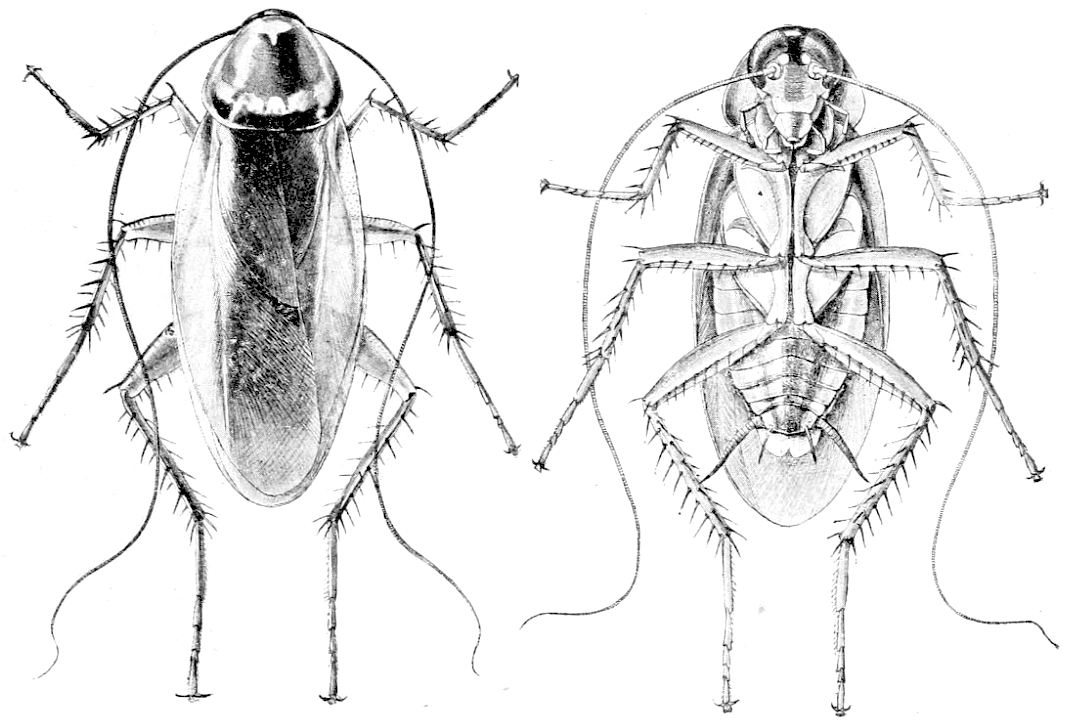
\includegraphics[width=0.6\textwidth]{BlattidHabitus}
  \caption{Blattidae, dorsal and ventral habitus \citep[][Fig. 1]{bhl129194}}
  \label{fig:blattid1}
\end{figure}

\subsection{Ectobiidae (was ``Blattellidae''; German cockroach, \textit{etc}.)}
\begin{itemize}
\item female subgenital plate not divided
\item male styli usually small, asymmetrical
\item spines on fore femur decrease in size apically
\end{itemize}

\begin{figure}[ht!]
    \centering
    \begin{subfigure}[ht!]{0.45\textwidth}
        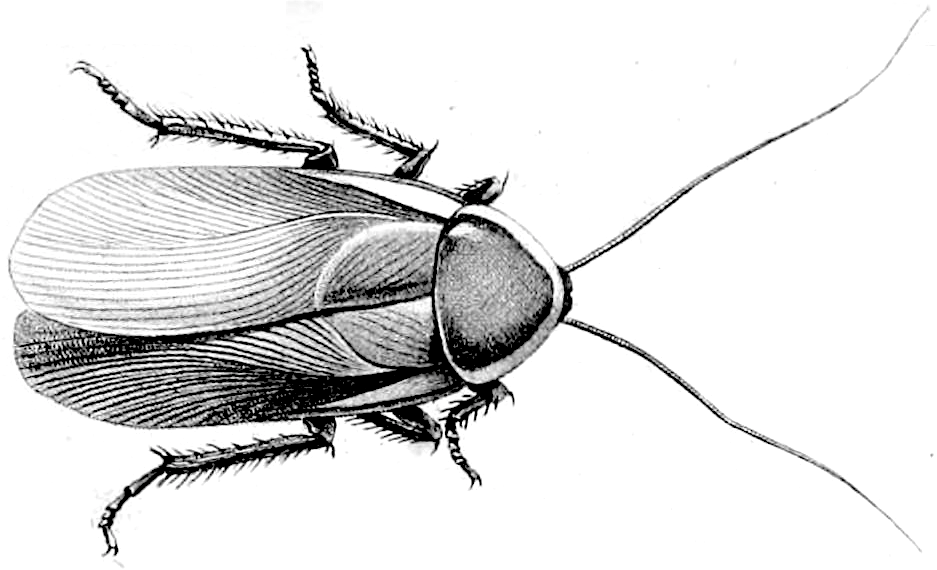
\includegraphics[width=\textwidth]{EctobiidHabitus}
        \caption{Habitus, dorsal \citep[][Plate III, Fig. 14A]{bhl26431}}
        \label{fig:ectobiidhabitus}
    \end{subfigure}
    \qquad
    \begin{subfigure}[ht!]{0.45\textwidth}
        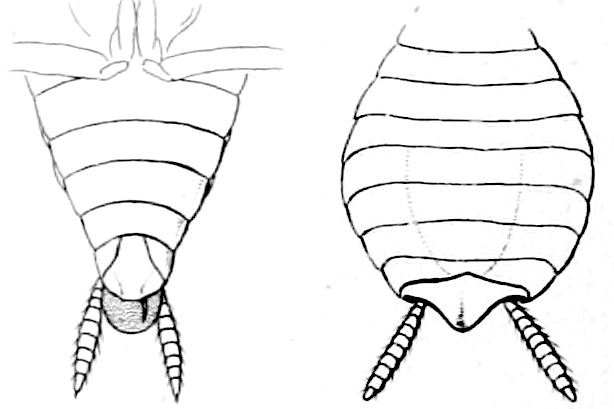
\includegraphics[width=\textwidth]{EctobiidAbdomen}
        \caption{Ventral view of abdomen apex; male (l), female (r) \citep[Plate II, Fig. 7E,D']{bhl26431}}
        \label{fig:ectobiidgenit}
    \end{subfigure}
    \caption{Ectobiidae}\label{fig:ectobiidae}
\end{figure}

\noindent{}Many insects are capable of walking or running quickly and efficiently. Why do you think cockroaches serve as the primary model for hexapodous robots? Is there something special about their morphology, or is the reason simpler than that?\vspace{4cm}

\subsection{Cryptocercidae (hooded cockroaches)}
\begin{itemize}
\item end of abdomen covered by 7th tergite dorsally, 6th sternite ventrally
\item no subgenital plate
\item always wingless
\item middle and hind femora with few spines relative to other families
\end{itemize}

\begin{figure}[ht!]
  \centering
    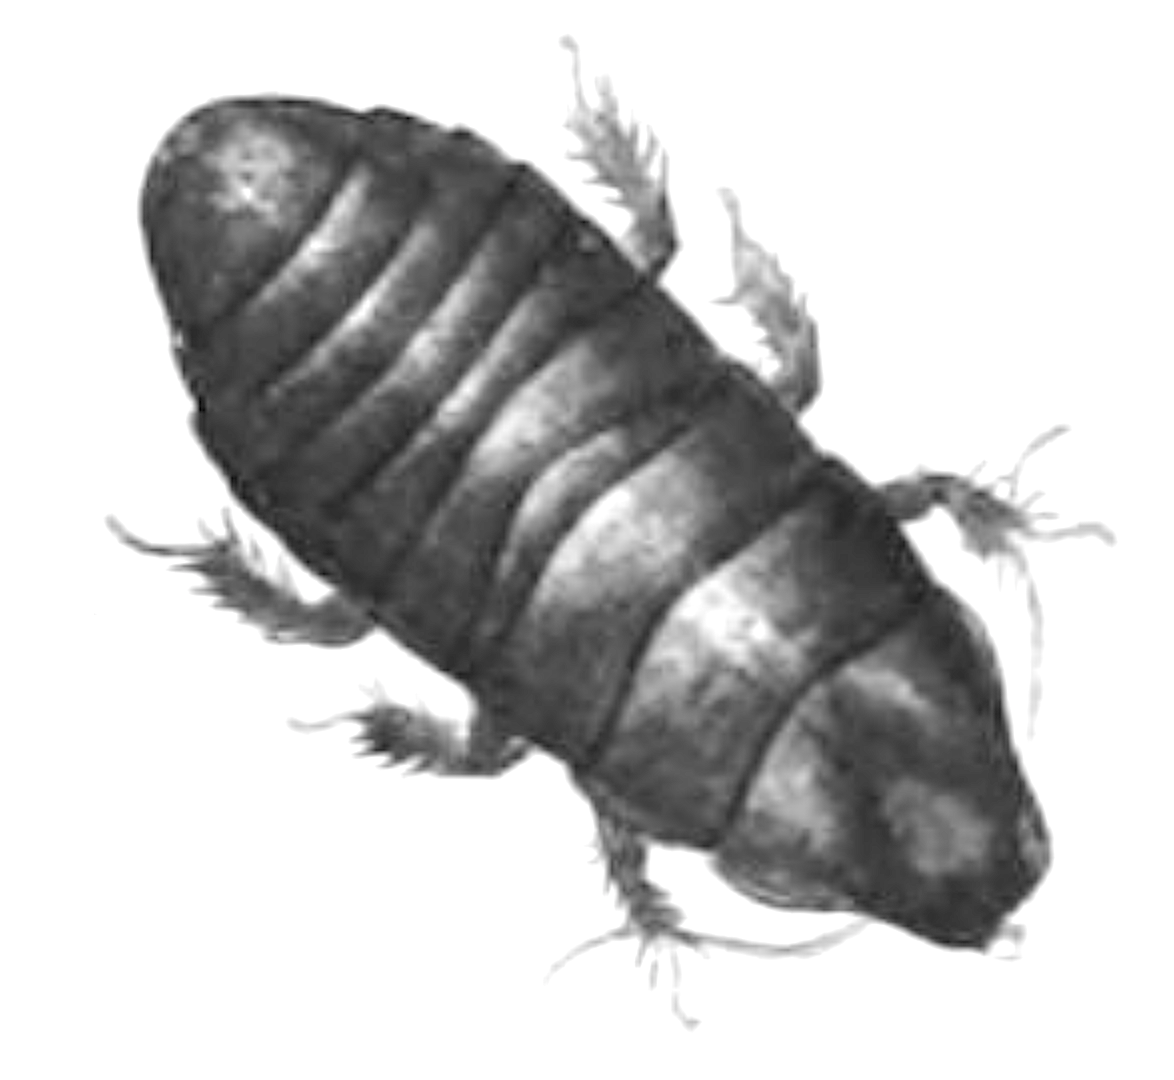
\includegraphics[width=0.3\textwidth]{CryptocercidHabitus}
  \caption{Cryptocercidae dorsal habitus \citep[][Plate VI, Fig. 20]{bhl18655}}
  \label{fig:cryptocercid}
\end{figure}

\subsection{Isoptera (termites)}
\begin{itemize}
\item pronotum not shield-like (Compare to other Blattodea!)
\item each tarsus subdivided into 4 tarsomeres (this character is difficult to see on dried specimen, please focus on glycerine-preserved specimens!)
\item cercus composed of 1--6 sclerites
\end{itemize}

\begin{figure}[ht!]
  \centering
    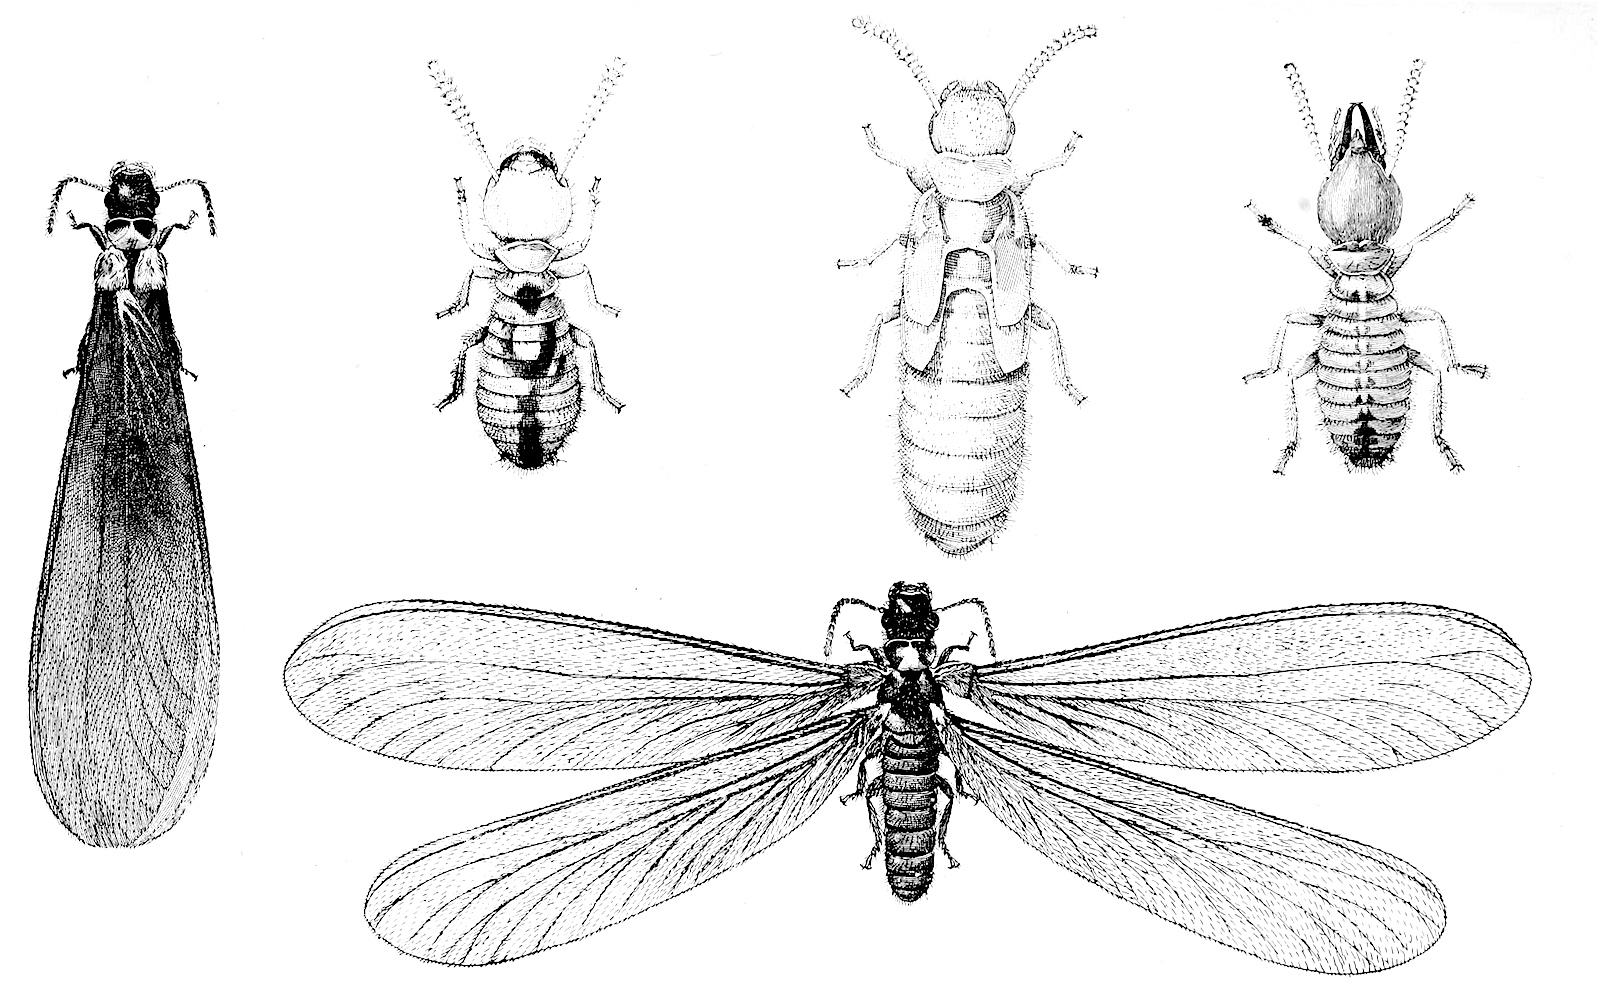
\includegraphics[width=0.7\textwidth]{Isoptera}
  \caption{Isoptera, alates, worker, soldier \citep[][Plate II]{bhl82061}}
  \label{fig:termite}
\end{figure}

\noindent{}The presence of a fontanelle (pore) on the head is used to diagnose families, as is the number of sclerotized wing veins along anterior margin of fore wing (\textit{e.g.}, two or three present). Can you find these features in our specimens? For soldiers, can you count the number of teeth on the inner margin of the left mandible?

\subsection{Mantodea}
\begin{itemize}
\item head roughly triangular, articulated with thorax via narrow neck (head highly mobile)
\item face with area (facial or frontal shield) delimited by carinae
\item prothorax elongate, with raptorial fore legs
\item fore wings (if present) = tegmina
\item male genitalia asymmetrical
\end{itemize}

\begin{figure}[ht!]
  \centering
    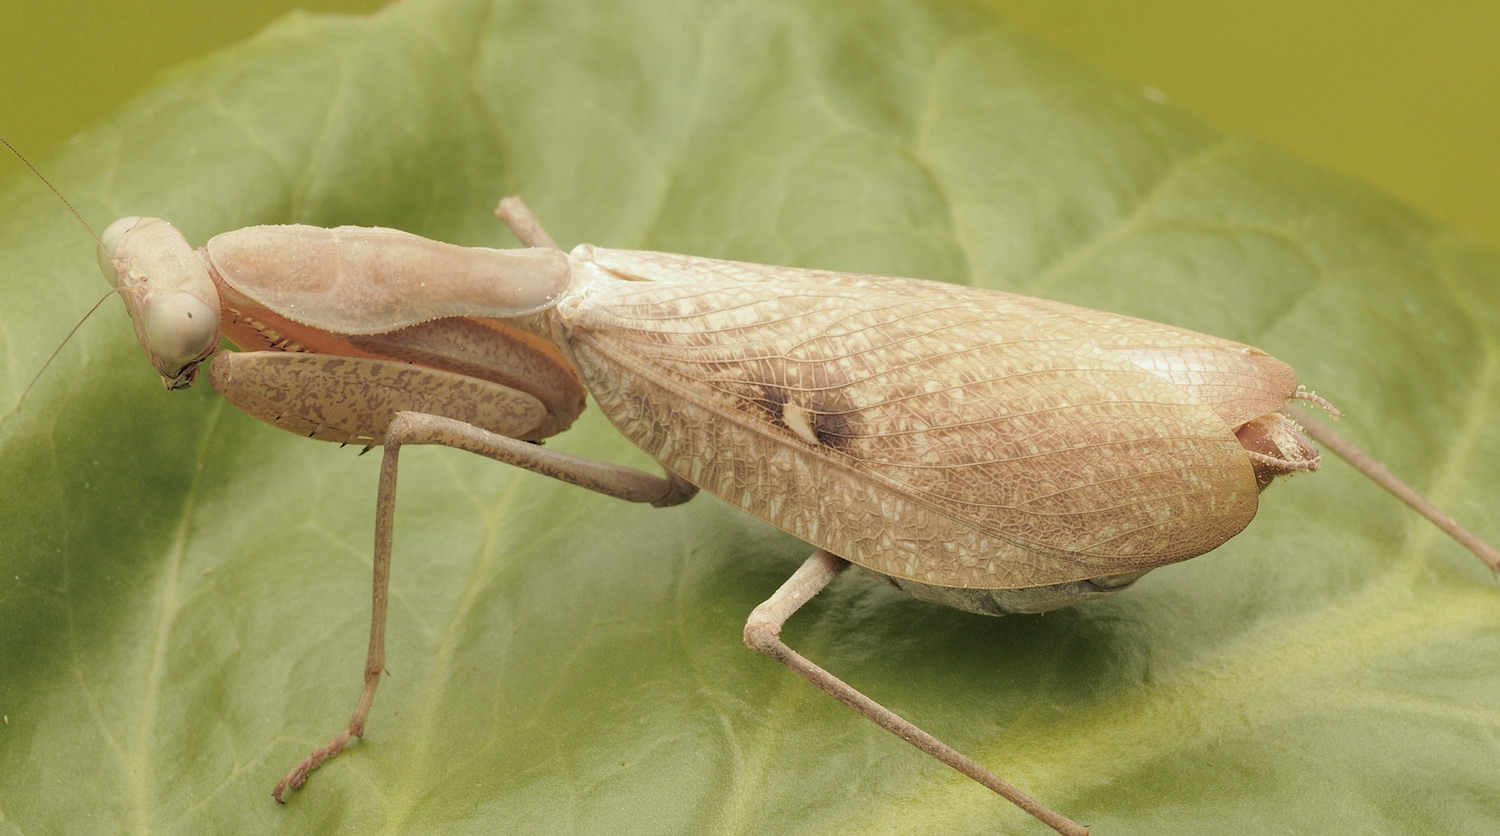
\includegraphics[width=0.7\textwidth]{mantid1}
  \caption{Mantodea. Photo (CC BY-ND 2.0) by Peter G. W. Jones \url{https://flic.kr/p/jjh5Hh}}
  \label{fig:mantidbody}
\end{figure}

\begin{figure}[ht!]
    \centering
    \begin{subfigure}[ht!]{0.35\textwidth}
        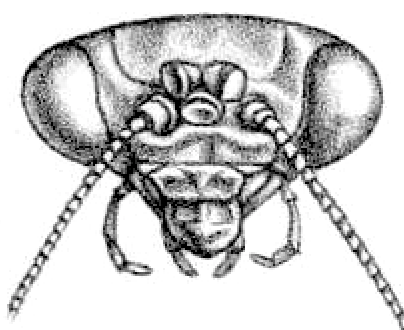
\includegraphics[width=\textwidth]{MantodeaHead}
        \caption{Head, anterior view \citep[modified from][Plate 130, Fig. 1a]{bhl24070}}
        \label{fig:mantodea1}
    \end{subfigure}
    \qquad
    \begin{subfigure}[ht!]{0.45\textwidth}
        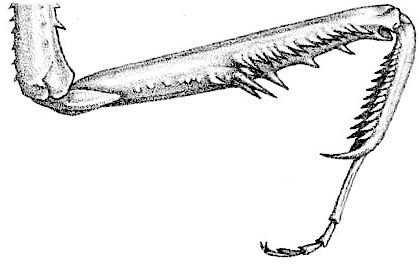
\includegraphics[width=\textwidth]{MantodeaForeLeg}
        \caption{Raptorial fore leg \citep[modified from][Plate 130, Fig. 1f]{bhl24070}}
        \label{fig:mantodea2}
    \end{subfigure}
    \caption{Mantodea}\label{fig:mantodeans}
\end{figure}

\section{Dermaptera (earwigs)}
\begin{itemize}
\item body dorsoventrally flattened
\item head prognathous
\item fore wings relatively short, heavily sclerotized, elytraform
\item hind wing fan-shaped
\item cerci forceps-like, each cercus comprised of a single segment
\item defensive glands open near 3rd and 4th abdominal tergites
\end{itemize}

\subsection*{Spongiphoridae (little earwigs; includes Labiidae)}
\begin{itemize}
\item 2nd tarsomere cylindrical
\item flagellum subdivided into 18--29 flagellomeres
\end{itemize}

\begin{figure}[ht!]
  \centering
    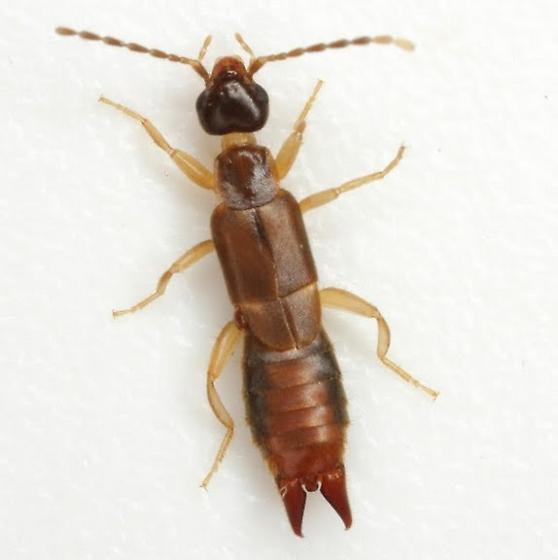
\includegraphics[width=0.5\textwidth]{spongi}
  \caption{\textit{Labia minor} (Spongiphoridae). Photo (CC BY-ND-NC 1.0) by Mike Quinn \url{http://bugguide.net/node/view/449544}}
  \label{fig:spongi}
\end{figure}

\subsection*{Forficulidae (European and spine-tailed earwigs)}
\begin{itemize}
\item 2nd tarsomere lobed apically
\item flagellum subdivided into 10--14 flagellomeres
\end{itemize}

\begin{figure}[ht!]
  \centering
    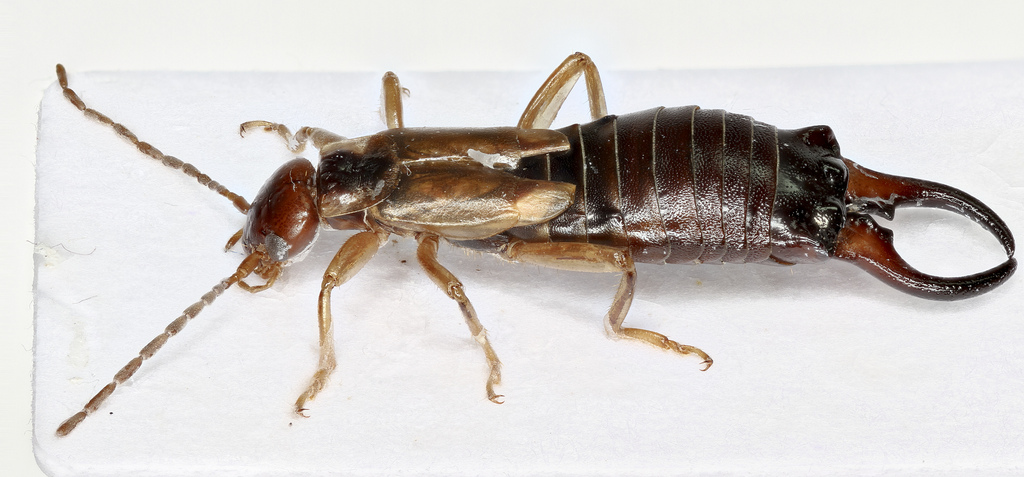
\includegraphics[width=0.75\textwidth]{forfic1}
  \caption{Forficulidae. Photo (CC BY-NC 2.0) by Chris Moody \url{https://flic.kr/p/eYFc5g}}
  \label{fig:forfic1}
\end{figure}

\section{Embioptera (webspinners, Embiodea, Embiidina)}
\begin{itemize}
\item body nearly cylindrical
\item head prognathous
\item proximalmost tarsomere greatly expanded to accommodate silk-producing glands
\item wings (males only) highly flexible, similar in size/shape
\item male genitalia asymmetrical
\end{itemize}

\begin{figure}[ht!]
  \centering
    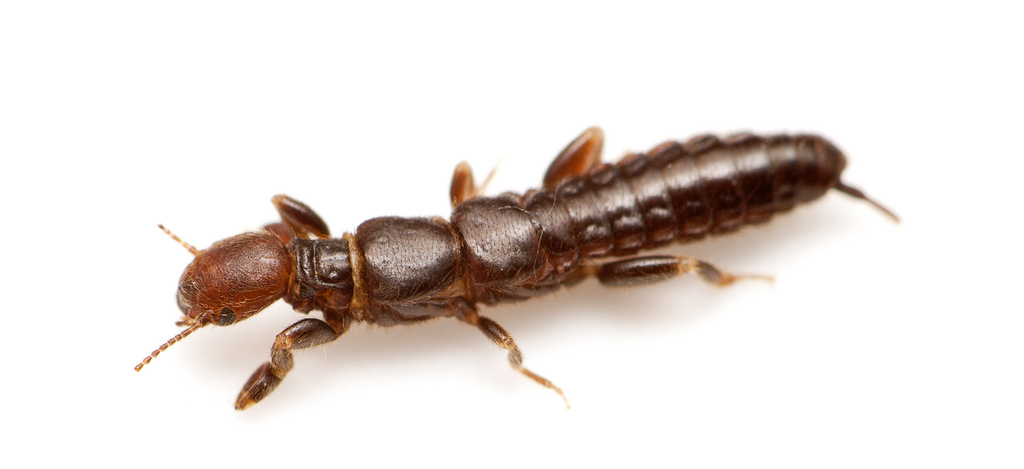
\includegraphics[width=0.85\textwidth]{embiop}
  \caption{Embioptera. Photo \textcopyright{ } by Matt Bertone \url{https://flic.kr/p/dEAs8y}}
  \label{fig:embiop1}
\end{figure}

\section{Orthoptera}
\begin{itemize}
\item head hypognathous
\item pronotum saddle-shaped
\item fore wing more sclerotized (tegmen) than hind wing
\item tarsus with 4 or fewer tarsomeres
\item hind leg saltatorial (femora enlarged)
\end{itemize}

\subsection*{Orthoptera: Caelifera}
\begin{itemize}
\item antenna usually less than half as long as body, 
\item flagellum subdivided into less than 28 flagellomeres 
\item tarsi subdivided into 3 or fewer tarsomeres
\item auditory organ is absent from the foreleg and usually present on the first abdominal segment.
\item ovipositor short
\end{itemize}

\subsubsection*{Tridactylidae (pygmy mole crickets)}
\begin{itemize}
\item pronotum does not extend over the length of the abdomen
\item fore and middle tarsi with 2 tarsomeres 
\item fore wing reduced, stridulatory organ absent
\item hind tarsus absent or represented by one tarsomere, shorter than apical hind tibial spurs; notice anything unusual about the phenotype of the hind leg?
\item body usually less than 20 mm long
\item auditory organ usually present on 1st abdominal segment; do pygmy mole crickets have 4 cerci?
\end{itemize}
%https://flic.kr/p/8Bs1y
\begin{figure}[ht!]
  \centering
    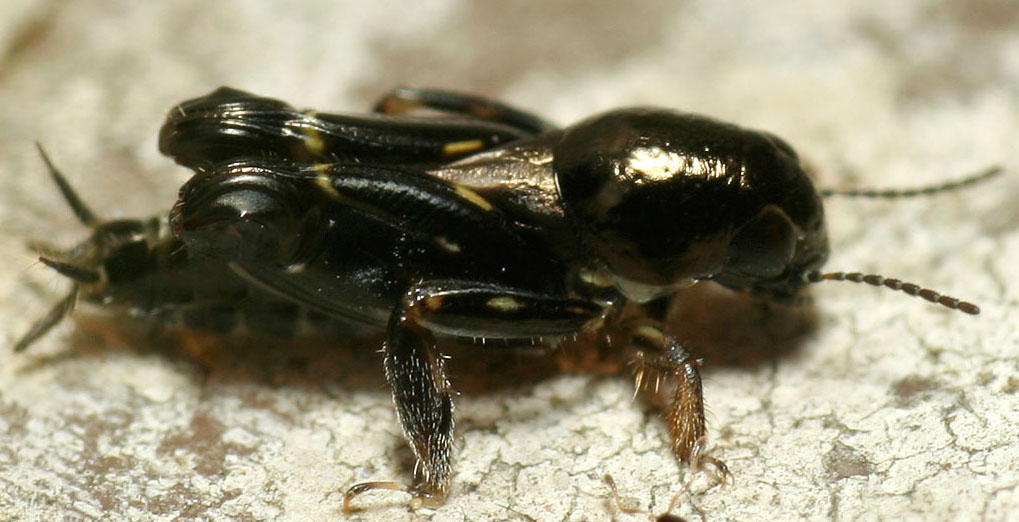
\includegraphics[width=0.7\textwidth]{tridact}
  \caption{Tridactylidae. Photo (CC BY-ND 2.0) by Gerald Yuvallos: \url{https://flic.kr/p/8Bs1y}}
  \label{fig:tridact}
\end{figure}
\vspace{3cm}
\subsubsection*{Tetrigidae (pygmy grasshoppers)}
\begin{itemize}
\item pronotum extended posteriorly largely overlaps hind wing and extends over the length of abdomen
\item hind tarsus with more than one tarsomeres (tarsomere formula = 2:2:3)
\item hind tarsus is longer than apical hind tibial spurs
\item body usually less than 20 mm long
\item fore wings are absent or vestigial
\item auditory organ absent
\end{itemize}

\noindent{}What is the function of the elongate pronotum? Is this structure perhaps taking over the function of another structure that is missing or reduced?\vspace{3cm}

\noindent{}Why don't these insects need auditory organs?\vspace{3cm}

\begin{figure}[ht!]
  \centering
    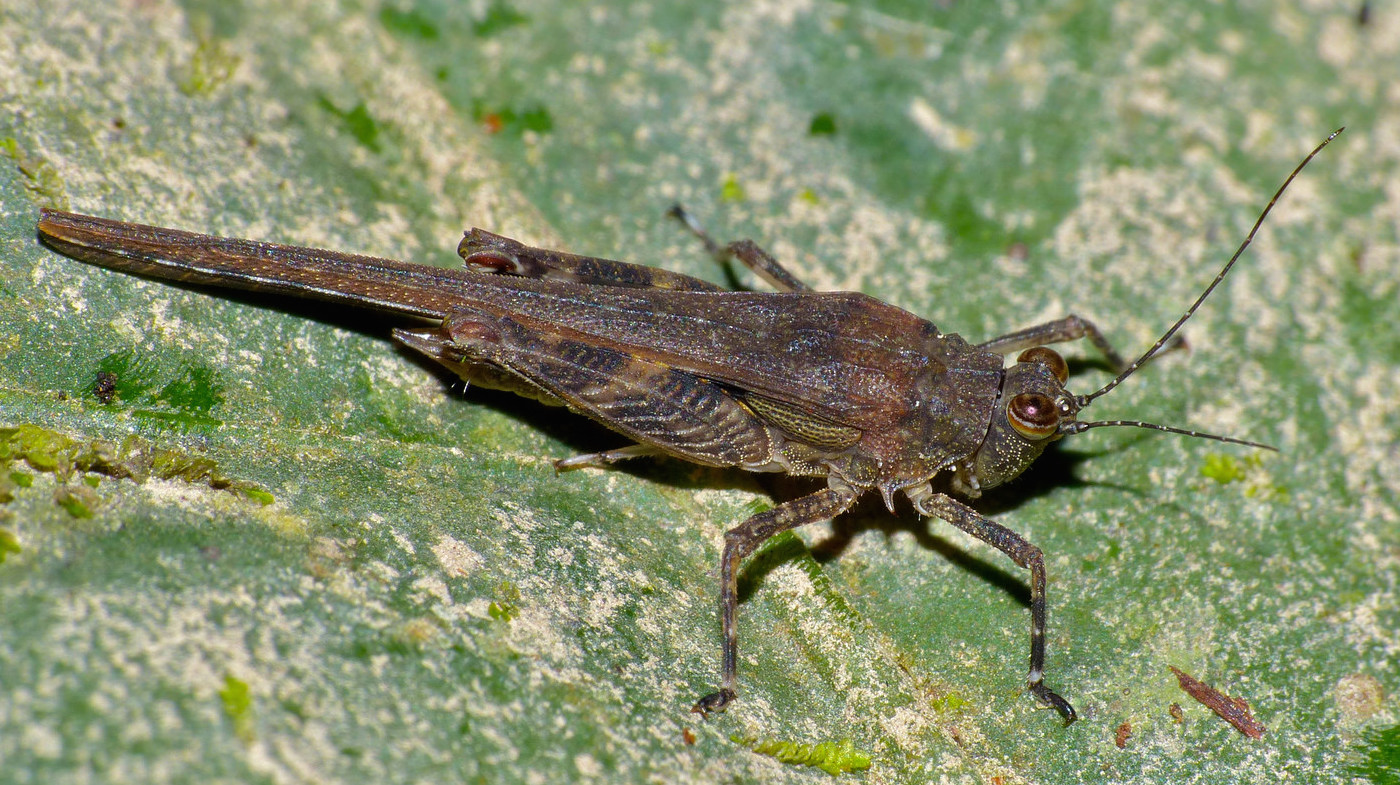
\includegraphics[width=0.75\textwidth]{tetrig1}
  \caption{Tetrigidae. Photo (CC BY-SA 2.0) by Bernard DuPont: \url{https://flic.kr/p/pBQHhe}}
  \label{fig:tetrig}
\end{figure}
%https://flic.kr/p/pBQHhe

\subsubsection*{Acrididae (short-horned grasshoppers)}
\begin{itemize}
\item pronotum not extended posteriorly, barely overlaps hind wing and does not extend over the length of the abdomen
\item fore wing well developed
\item hind tarsus with more than one tarsomere (each tarsus with 3 tarsomeres)
\item hind tarsus is longer than apical hind tibial spurs
\item body usually more than 20 mm long
\item auditory organ usually present laterally on 1st abdominal segment
\end{itemize}

\noindent{}Grasshoppers have ears so that they can listen to each other. How do they make sounds?\vspace{3cm}

\begin{figure}[ht!]
  \centering
    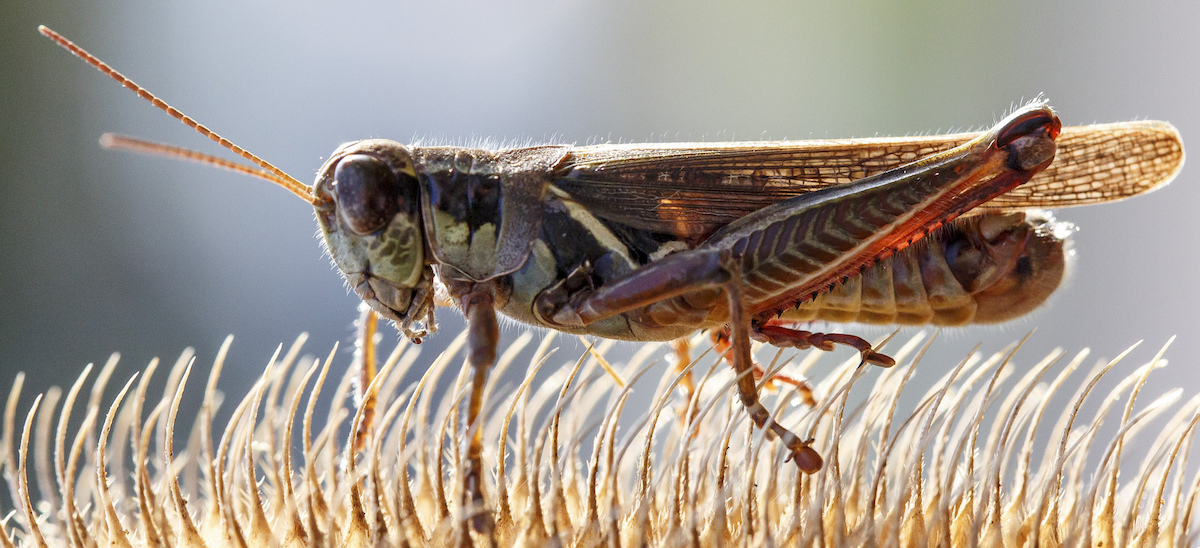
\includegraphics[width=0.75\textwidth]{acrid}
  \caption{Acrididae. Photo (CC BY-NC-ND 2.0) by Richard Ricciardi \url{https://flic.kr/p/pt7Cxc}}
  \label{fig:acrididhabitus}
\end{figure}

\subsection*{Orthoptera: Ensifera (crickets, katydids)}
\begin{itemize}
\item antennae usually more than half as long as body, composed of more than 30 antennal sclerites
\item tarsi with 3--4 tarsomeres
\item auditory organ is usually present on the fore leg; can you locate this organ and compare with the auditory organ of Caelifera?
\item ovipositor long
\end{itemize}

\subsubsection*{Tettigoniidae (long-horned grasshoppers, katydids)}
\begin{itemize}
\item tarsus with 4 tarsomeres
\item antennal foramina widely separated from each other
\item fore wing held roof-like over abdomen
\item ovipositor sword-shaped, usually curved
\item hind tibia with equally-sized spines
\item auditory organs present on front tibiae
\end{itemize}

\begin{figure}[ht!]
  \centering
    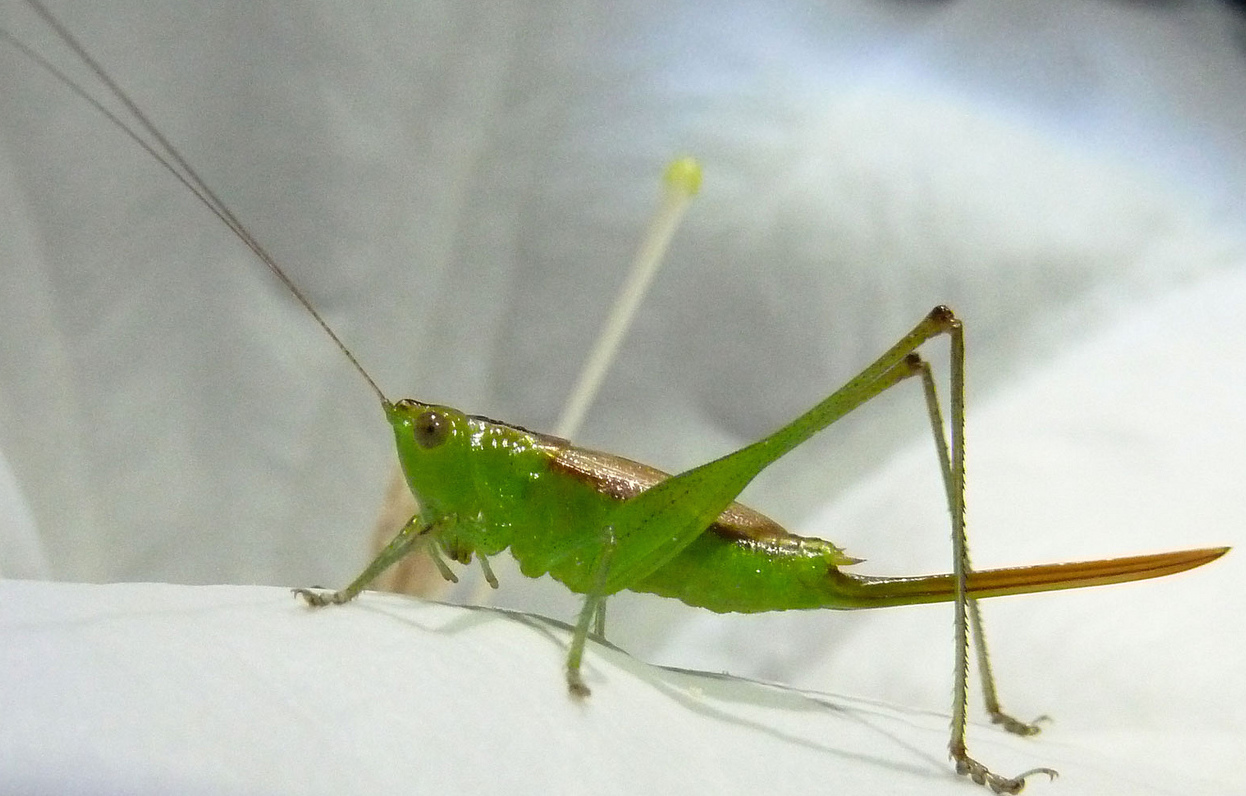
\includegraphics[width=0.75\textwidth]{tetti1}
  \caption{Tettigoniidae. Photo (CC BY 2.0) by Katja Schulz \url{https://flic.kr/p/cY9v5G}}
  \label{fig:tettihabitus}
\end{figure}

\noindent{}Katydids have their ears in a very different part of their bodies, compared to grasshoppers. Do they also make sounds in different ways? \vspace{3cm}

\begin{figure}[ht!]
  \centering
    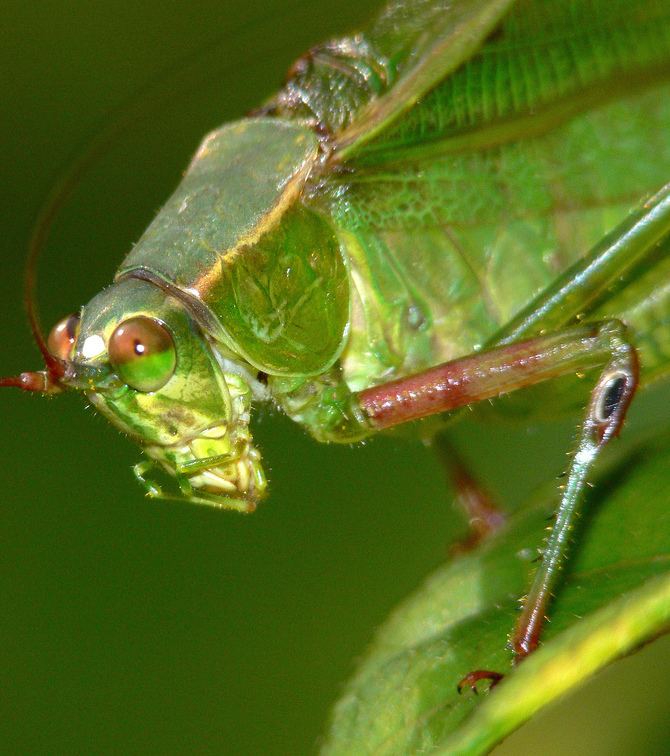
\includegraphics[width=0.55\textwidth]{tetti2}
  \caption{Tettigoniidae. Photo (CC BY-NC 2.0) by Brad Smith \url{https://flic.kr/p/oCdoi}}
  \label{fig:tettihead}
\end{figure}

\subsubsection*{Rhaphidophoridae (camel crickets)}
\begin{itemize}
\item mid tarsus subdivided into 4 tarsomeres, others 4 or 3
\item antennal foramina contiguous
\item wingless, usually humpbacked in appearance
\item ovipositor sword-shaped, usually curved
\item hind tibia with equally sized spines
\item auditory organ on fore tibia usually absent
\item pseudotympanum on abdomen present
\end{itemize}

\noindent{}Why don't these insects need an ear?\vspace{3cm}

\begin{figure}[ht!]
  \centering
    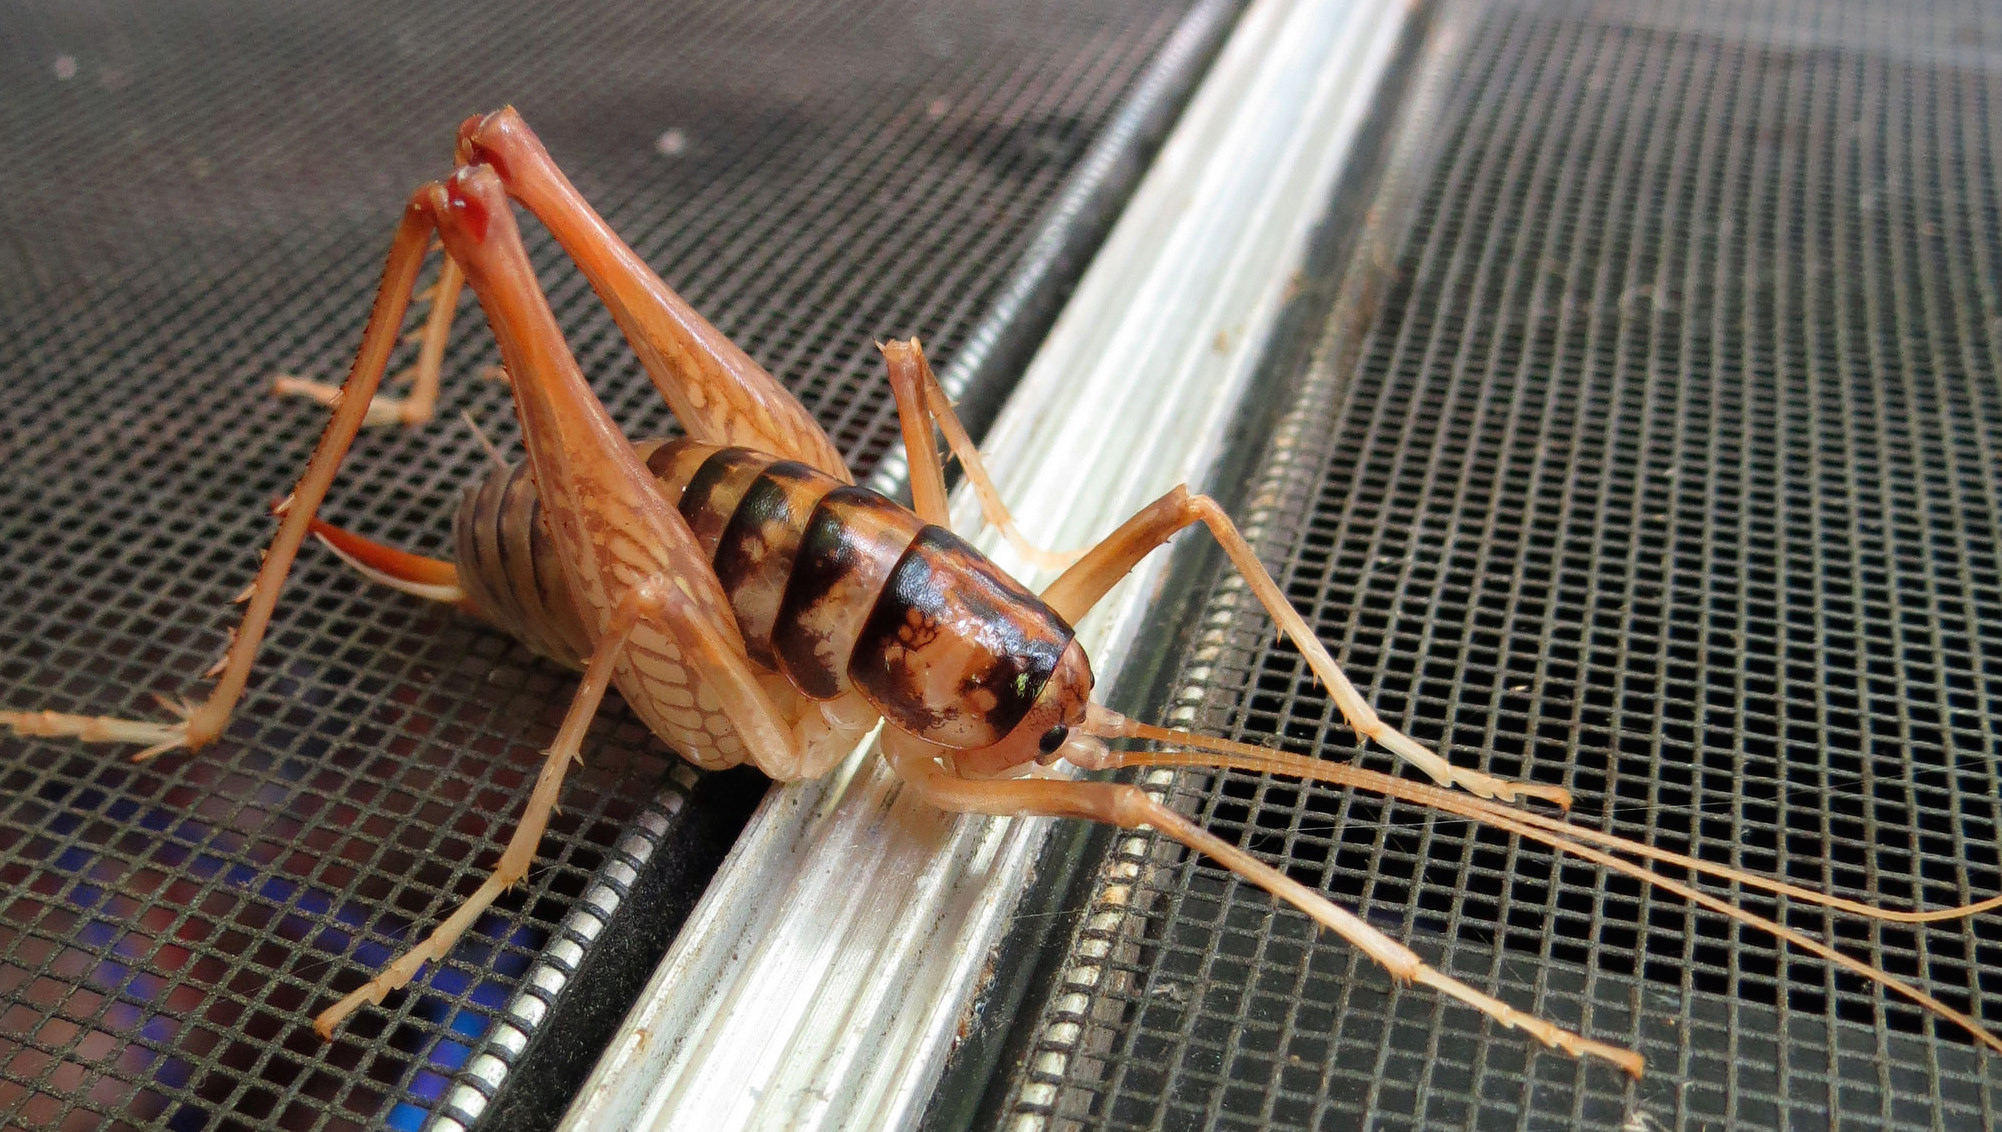
\includegraphics[width=0.75\textwidth]{rhaphid}
  \caption{Rhaphidophoridae. Photo (CC BY 2.0) by Katja Schulz \url{https://flic.kr/p/ouPNVx}}
  \label{fig:rhaphid}
\end{figure}

\subsubsection*{Gryllidae (crickets, tree crickets)}
\begin{itemize}
\item tarsi subdivided into 3 tarsomeres
\item antennal foramina widely separated from each other
\item wings flattened on back, not roof-like 
\item male fore wing with ``harp''
\item ovipositor cylindrical, not curved
\item auditory organ on fore tibia present
\end{itemize}

\begin{figure}[ht!]
  \centering
    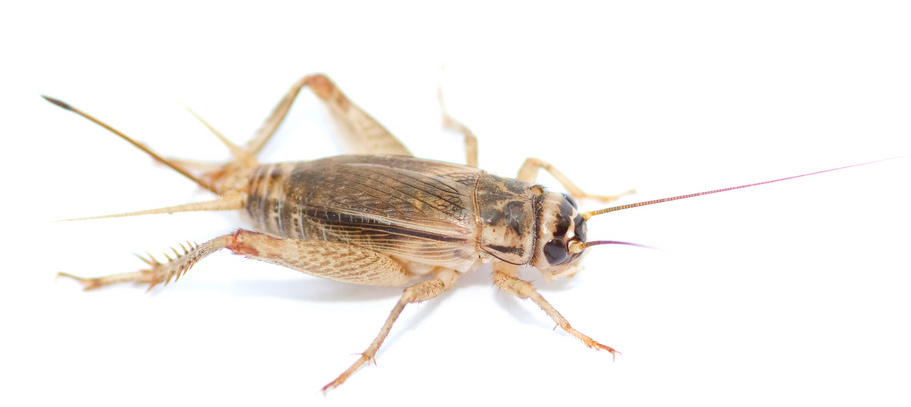
\includegraphics[width=0.85\textwidth]{gryll}
  \caption{Gryllidae. Photo (CC BY 2.0) by Brian Gratwicke \url{https://flic.kr/p/7XHo1E}}
  \label{fig:gryllid}
\end{figure}

\subsubsection*{Gryllotalpidae (mole crickets)}
\begin{itemize}
\item tarsi subdivided into 3 tarsomeres 
\item antennal foramina widely separated from each other
\item wings flattened on back, not rooflike 
\item male fore wing with ``harp''
\item fore leg fossorial 
\item ovipositor short
\item hind tibia with alternating sized spines
\item auditory organ on fore tibia usually present
\item pseudotympanum on abdomen present; can you locate this organ? Why is it called ``pseudo'' tympanum?
\end{itemize}
\vspace{4cm}
\begin{figure}[ht!]
  \centering
    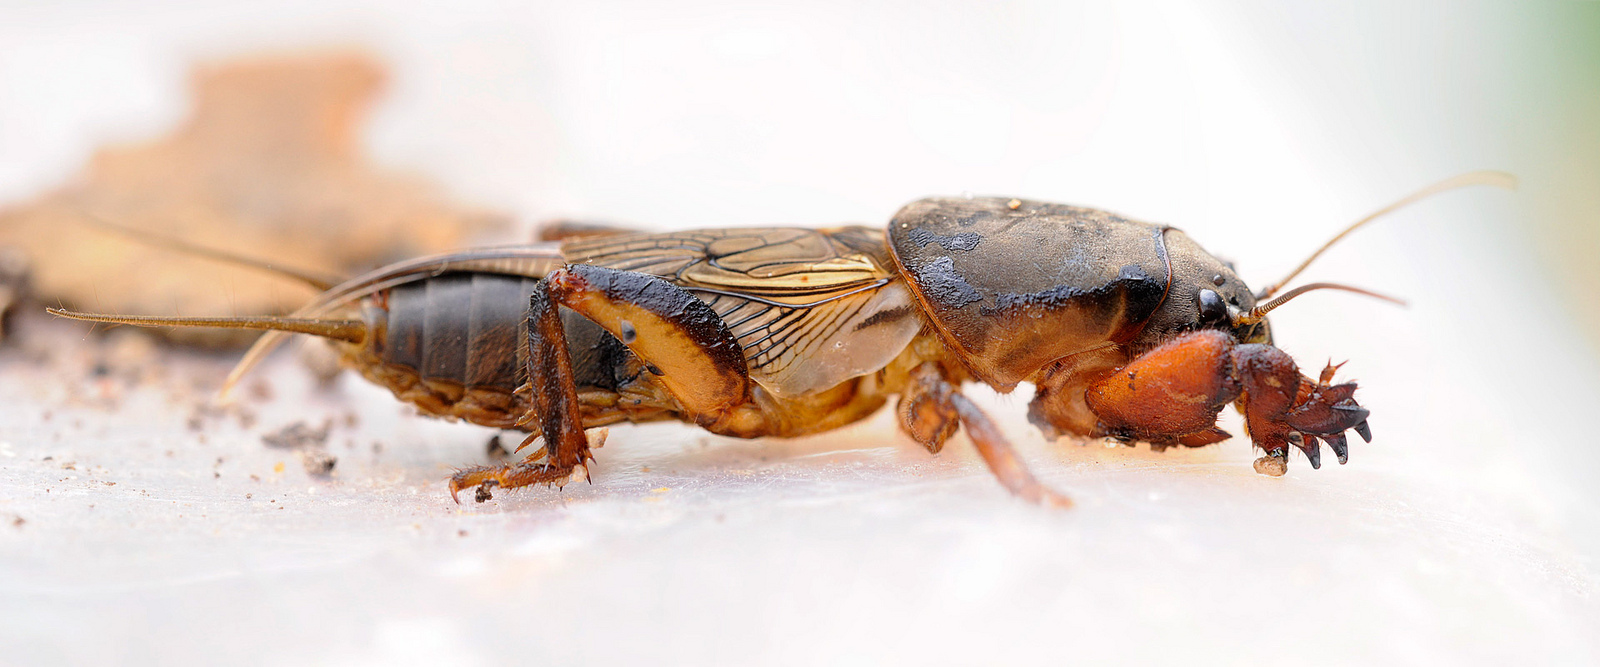
\includegraphics[width=0.85\textwidth]{gryllotalp}
  \caption{Gryllotalpidae. Photo (CC BY-NC-ND 2.0) by Sergey Yeliseev \url{https://flic.kr/p/eGcrxX}}
  \label{fig:gryllotalp}
\end{figure}

\section{Phasmatodea (Phasmida; walking sticks, leaf insects)}
\begin{itemize}
\item frons anterolaterally convex
\item prothroax with defensive gland openings
\item trochanter+femur nearly fused
\end{itemize}

\subsection*{Heteronemiidae (common walkingsticks)}
\begin{itemize}
\item mesothorax at least 4 times as long as prothorax
\item each leg with 5 tarsomeres
\item head without spines posteriorly
\item 1st abdominal segment shorter than metathorax
\item usually wingless
\end{itemize}

\begin{figure}[ht!]
  \centering
    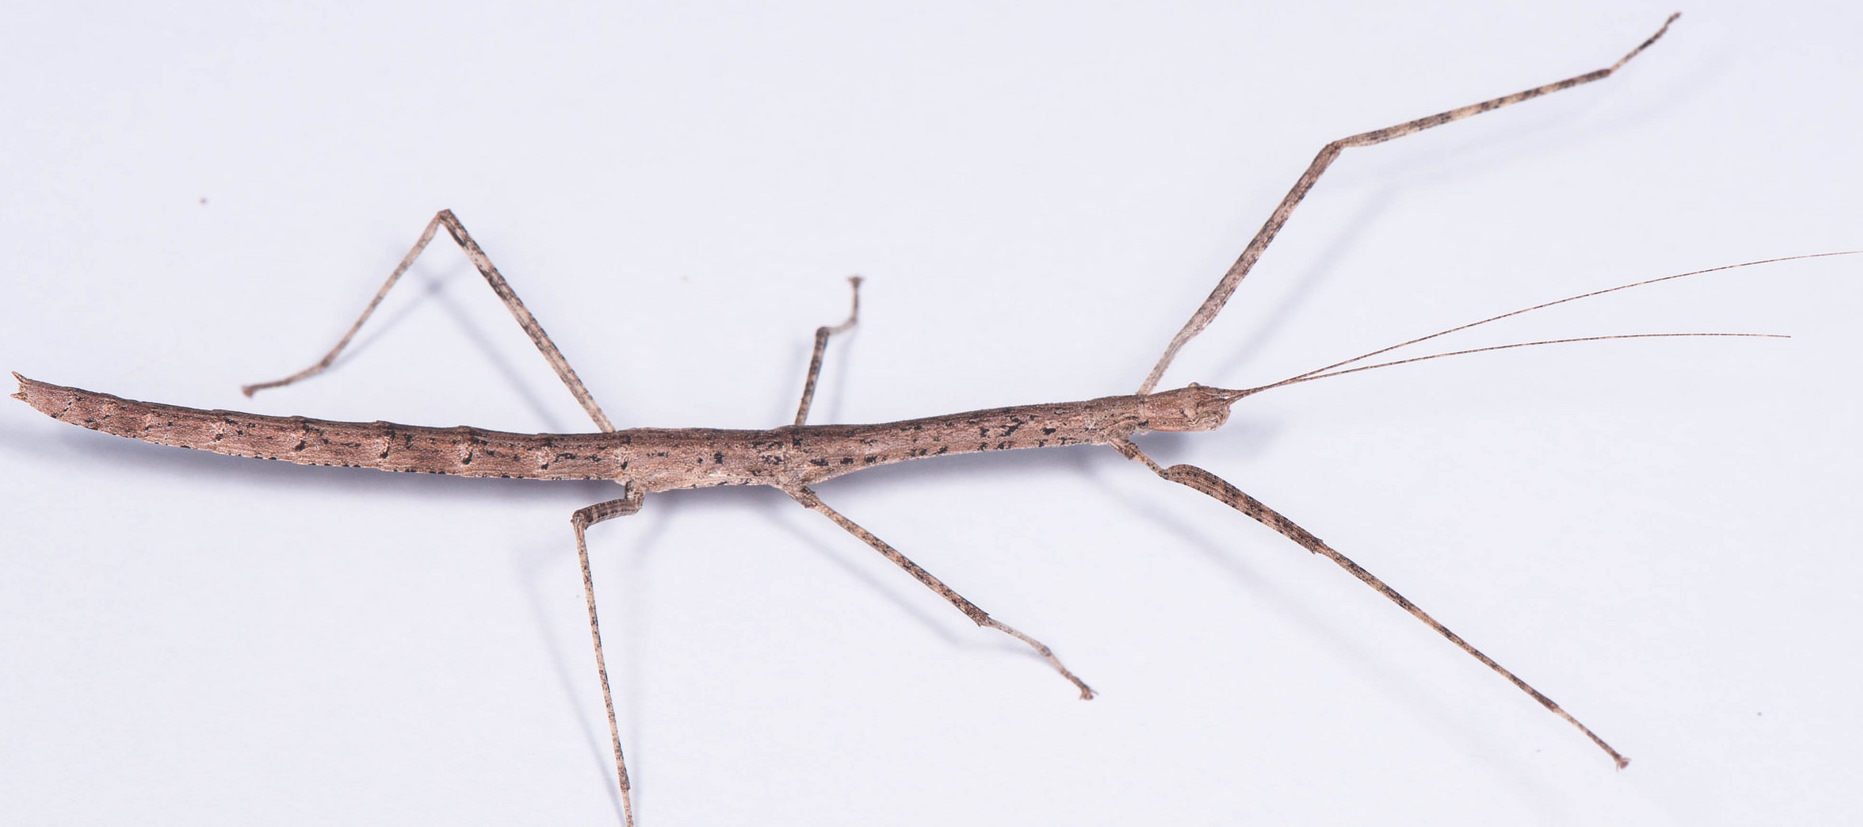
\includegraphics[width=0.85\textwidth]{phasma}
  \caption{Heteronemiidae. Photo (CC BY-NC-ND 2.0) by Mark Yokoyama \url{https://flic.kr/p/skW7zQ}}
  \label{fig:heteronemiid}
\end{figure}

\section{Grylloblattodea (ice crawlers)}
\subsection*{Grylloblattidae}
\begin{itemize}
\item head prognathous
\item compound eyes reduced or absent
\item wings absent
\item cerci multi-segmented
\end{itemize}

\begin{figure}[ht!]
  \centering
    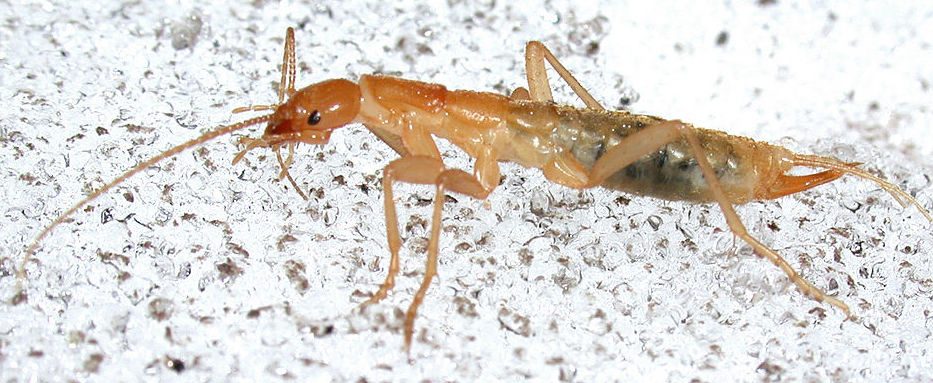
\includegraphics[width=0.85\textwidth]{grylloblattidae}
  \caption{Grylloblattodea. Photo (CC0) by Alex Wild \url{https://commons.wikimedia.org/wiki/File:Grylloblattidae.jpg}}
  \label{fig:grylloblatt}
\end{figure}

\section{Mantophasmatodea (heel-walkers, gladiators)}

\noindent{}Unfortunately, we do not have any specimens of this taxon, which lives in southern Africa.
\begin{itemize}
\item head hypognathous
\item antennae long, with spindle-shaped flagellomeres distally
\item arolium (pad-like structure on the distal end of each leg) expanded, held aloft when moving
\item legs adapted for grabbing prey (spiny)
\item wingless
\end{itemize}

\noindent{}Although they are relatively common, heel-walkers were only discovered recently (2001). Why did researchers overlook members of this taxon for so long? 

\begin{figure}[ht!]
  \centering
    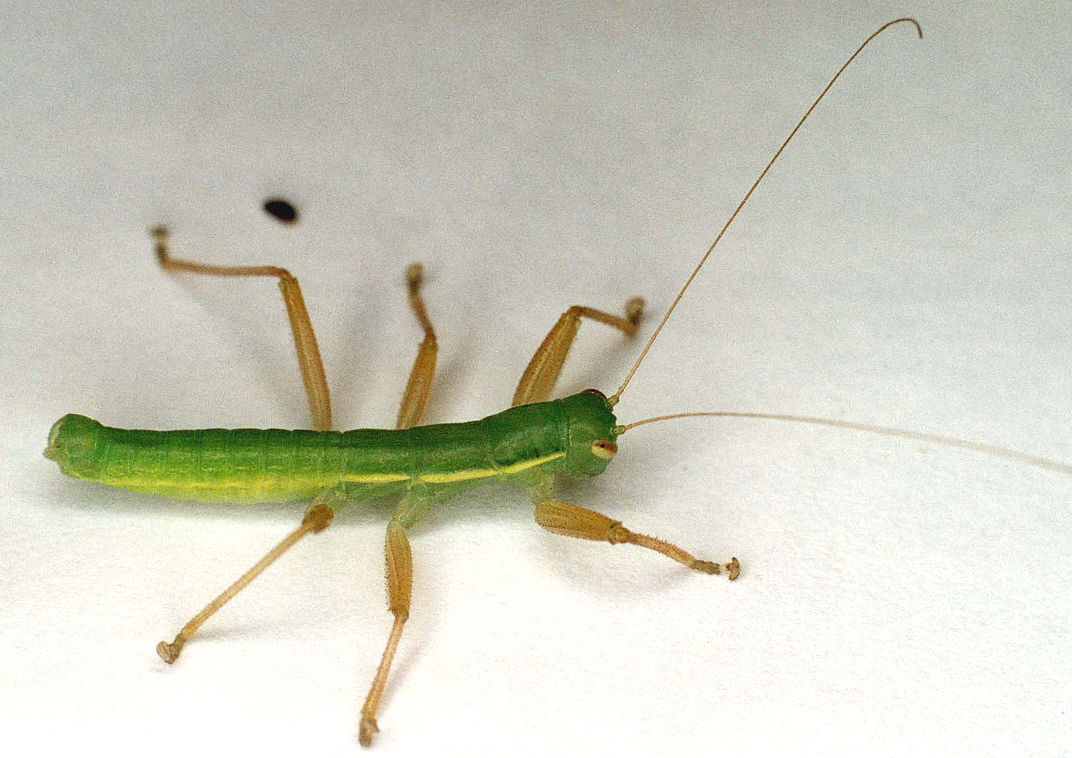
\includegraphics[width=0.75\textwidth]{mantophas}
  \caption{Mantophasmatodea. Photo (CC BY-SA 3.0) by P.E. Bragg \url{http://bit.ly/1WcySdc}}
  \label{fig:mantophas}
\end{figure}

\section{Zoraptera}

\noindent{}Note that these insects are gregarious, and the overall phenotype of an individual depends on status of the aggregation.
\begin{itemize}
\item pale, eyeless, wingless OR
\item pigmented (brown), with small compound eyes and wings (wings are dehiscent though!); wings with relatively simple venation
\item tarsus with 2 tarsomeres
\item cerci comprised of one apparent segment (\textit{i.e.}, no subdivisions)
\end{itemize}

\noindent{}There is one extant family: Zorotypidae.

\begin{figure}[ht!]
    \centering
    \begin{subfigure}[ht!]{0.45\textwidth}
        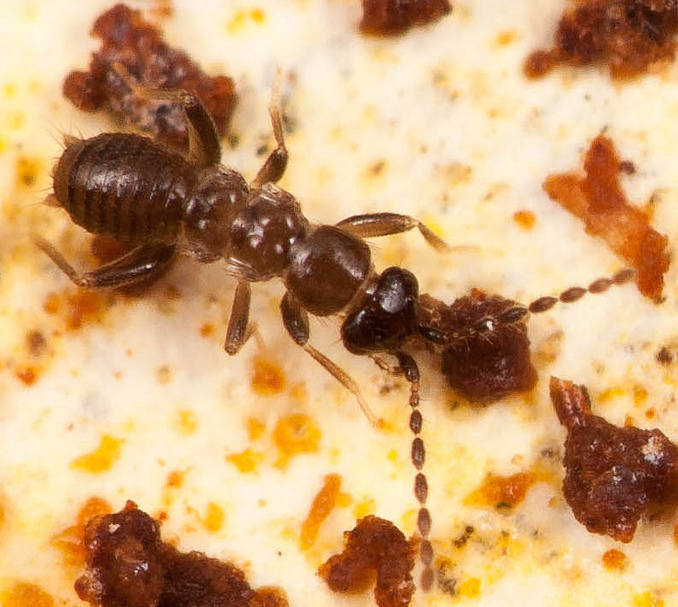
\includegraphics[width=\textwidth]{zorap1}
        \caption{Zorapteran with eyes; wings have fallen off. Photo \textcopyright{} by Matt Bertone \url{https://flic.kr/p/dgJ1iJ}}
        \label{fig:zorapbrown}
    \end{subfigure}
    ~ %add desired spacing between images, e. g. ~, \quad, \qquad, \hfill etc. 
      %(or a blank line to force the subfigure onto a new line)
    \begin{subfigure}[ht!]{0.45\textwidth}
        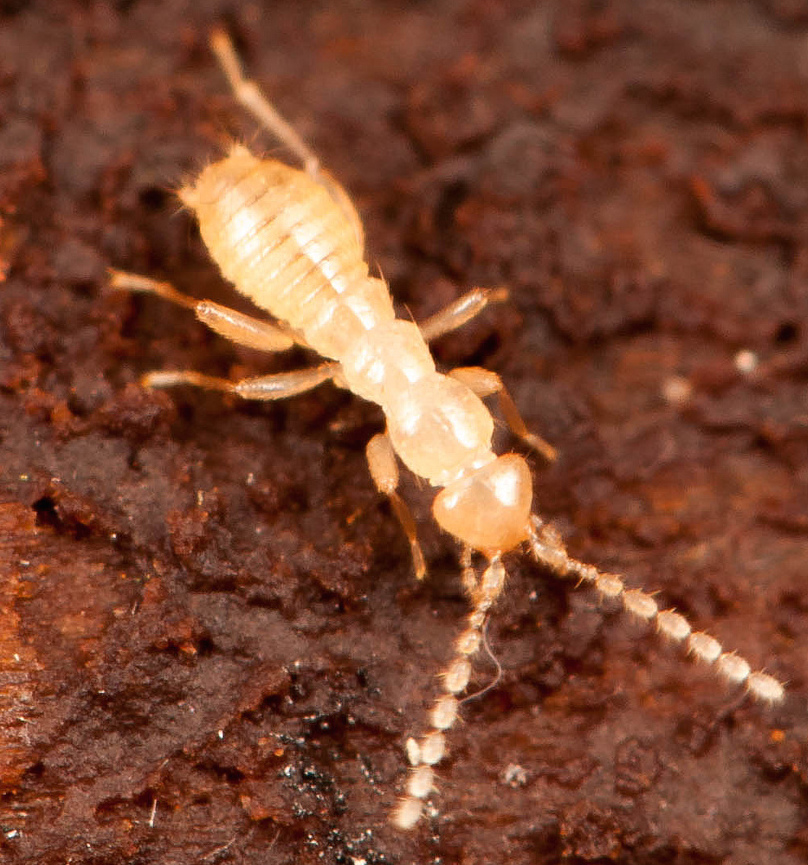
\includegraphics[width=\textwidth]{zorap2}
        \caption{Whitish, eyeless zorapteran. Photo \textcopyright{} by Matt Bertone \url{https://flic.kr/p/dgJ1vo}}
        \label{fig:zorapwhite}
    \end{subfigure}
    \caption{Zoraptera}\label{fig:zorapterans}
\end{figure}

\FloatBarrier

\section*{Acknowledgments}
Andrew R. Deans and Istv\'an Mik\'o wrote the text. Many of the illustrations were generously made available by the Biodiversity Heritage Library (\url{http://biodiversitylibrary.org}) and the photographers at Flickr (\url{http://flickr.com}).

\FloatBarrier
% adding bibliography here
\bibliographystyle{apalike}
\bibliography{bib}

\end{document}